\documentclass[11pt,a4paper]{article}

% --- Codificación e idioma ---
\usepackage[utf8]{inputenc}
\usepackage[T1]{fontenc}
\usepackage[spanish, es-tabla]{babel}

% --- Paquetes matemáticos ---
\usepackage{amsmath}
\usepackage{amssymb}

% --- Tipografía: Times New Roman---
\usepackage{mathptmx}

% --- Márgenes: 2.5 cm en todos los lados---
\usepackage[a4paper, margin=2.5cm]{geometry}

% --- Interlineado: 1.5 líneas---
\usepackage{setspace}
\onehalfspacing

% --- Formato de títulos y subtítulos---
\usepackage{titlesec}
\titleformat{\section}
  {\fontsize{16}{20}\selectfont\bfseries}
  {\thesection}{1em}{}
\titleformat{\subsection}
  {\fontsize{14}{18}\selectfont\bfseries}
  {\thesubsection}{1em}{}
\titleformat{\subsubsection}
  {\fontsize{12}{15}\selectfont\bfseries}
  {\thesubsubsection}{1em}{}

% --- Carátula UBA (DC/Exactas) ---
\usepackage[sinEntregas]{latex/caratula}

% --- Tablas profesionales ---
\usepackage{booktabs}
\usepackage{array}
\usepackage{caption}
\captionsetup{font=small, labelfont=bf, skip=8pt}

% --- Hipervínculos ---
\usepackage{hyperref}
\hypersetup{
    colorlinks=true,
    linkcolor=black,
    citecolor=blue,
    urlcolor=blue
}

\begin{document}

% ==============================================================================
% 1. CARÁTULA
% ==============================================================================
\pagenumbering{gobble} % Sin número de página en la carátula

\titulo{Análisis Microclimático y Riesgo Biológico en Salas de Colecciones del MACN}
\subtitulo{Modelado del efecto climático exterior sobre la temperatura interna y la proliferación de plagas}

\fecha{\today}
\materia{Casos de Estudio en Estadística}
\submateria{Solicitante: Área de Conservación Preventiva (MACN)}
\grupo{Grupo 42}

% Integrantes del grupo (Nombre, LU, email)
\integrante{Calo, Agustín}{LU2}{email2@ejemplo.com}
\integrante{Cogno, Matías}{LU2}{email2@ejemplo.com}
\integrante{Bravo, Ivan Agustín}{LU2}{email2@ejemplo.com}
\integrante{Kiss, Delfina}{72/23}{kissdelfina@gmail.com}


\maketitle

\newpage
\pagenumbering{arabic} % Numeración arábiga desde el Resumen

% ==============================================================================
% 2. RESUMEN (Aproximadamente 1 página según pautas)
% ==============================================================================
\section{Resumen}

\textbf{Contexto y Problema:} La conservación preventiva de colecciones biológicas históricas depende críticamente de la estabilidad microclimática en las salas de guarda. Variaciones bruscas de temperatura o niveles elevados de humedad relativa pueden provocar fatiga estructural en los ejemplares o favorecer la proliferación de insectos perjudiciales (como coleópteros y lepidópteros de museos). En este trabajo se analiza el grado de acoplamiento térmico entre las condiciones meteorológicas exteriores registradas por el Servicio Meteorológico Nacional (SMN) y el microclima interno de diversas salas del Museo Argentino de Ciencias Naturales (MACN) y colecciones asociadas, evaluando asimismo la relación con las capturas de insectos en trampas de monitoreo.

\textbf{Metodología:} Se procesaron registros continuos de temperatura y humedad tomados con sensores HOBO en 14 sectores y salas. Para evitar inferencias espurias debidas a la fuerte autocorrelación temporal, se ajustaron modelos de mínimos cuadrados generalizados (GLS) con estructura autorregresiva de primer orden ($AR(1)$) y armónicos anuales. La inercia térmica de cada espacio se determinó mediante la comparación de ventanas de promedio móvil exterior. Paralelamente, se exploraron las tasas de captura de insectos mediante modelos para datos de conteo con offset temporal para estandarizar los intervalos de exposición.

\textbf{Principales Hallazgos:} Los resultados revelan dos regímenes térmicos bien diferenciados dentro del museo: (1) \textit{Salas permeables o expuestas} (e.g., Paleovertebrados Anexo y Arácnidos), caracterizadas por una rápida respuesta al exterior (inercia de 2 días), pendientes elevadas ($\beta \approx 0{,}50 - 0{,}62\,^\circ\text{C}_\text{int}/^\circ\text{C}_\text{ext}$) y una marcada amplitud térmica diaria; y (2) \textit{Salas aisladas o con alta inercia} (e.g., Ictiología Colección, Ornitología y Paleovertebrados Ameghino), que presentan una inercia de 4 a 7 días, menor transmisión de calor ($\beta \approx 0{,}07 - 0{,}17$) y una memoria propia dominante ($\phi > 0{,}90$). En cuanto al riesgo biológico, la tasa diaria de capturas de plagas exhibe una fuerte estacionalidad asociada a la temperatura ($p = 0{,}017$), observándose un incremento de la actividad en los meses estivales.

\textbf{Implicancias:} Los hallazgos permiten identificar qué sectores requieren intervención prioritaria en aislamiento pasivo o acondicionamiento climático activo, y justifican el establecimiento de calendarios de monitoreo y control de plagas intensificados al comienzo de la temporada estival.

\newpage

% ==============================================================================
% 3. INTRODUCCIÓN Y OBJETIVOS
% ==============================================================================
\section{Introducción y Objetivos}

Las colecciones de historia natural albergan bienes culturales y científicos irremplazables cuya preservación a largo plazo está condicionada por el ambiente de guarda...

\subsection{Preguntas de investigación e hipótesis}
\begin{enumerate}
    \item ¿En qué medida y con qué retardo temporal penetran las fluctuaciones meteorológicas exteriores en las salas del museo?
    \item ¿Presentan todas las salas el mismo nivel de aislamiento o existen diferencias edilicias sustanciales?
    \item ¿Se observa una correlación entre el microclima y la proliferación de insectos plaga en las colecciones?
\end{enumerate}

% ==============================================================================
% 4. METODOLOGÍA
% ==============================================================================
\section{Metodología}

\subsection{Fuente de datos}
Se utilizaron dos fuentes de datos principales:
\begin{itemize}
    \item \textbf{Exterior:} Datos meteorológicos diarios de la estación Buenos Aires Observatorio Central (OMM 87585) del Servicio Meteorológico Nacional (SMN).
    \item \textbf{Interior:} Registros periódicos de temperatura, humedad relativa y punto de rocío obtenidos mediante dataloggers HOBO.
    \item \textbf{Biológico:} Registros de capturas en trampas de monitoreo de coleópteros y lepidópteros en las salas MACN-Ba, MACN-En y MACN-Ma.
\end{itemize}

\subsection{Procesamiento y limpieza de datos}
Se eliminaron los registros de bordes (primer y último día de muestreo de cada despliegue) por tratarse de días incompletos. Asimismo, se corrigió la identificación de dataloggers superpuestos en series complejas como Ornitología (diferenciando las colecciones Antigua y Azara)...

\subsection{Estrategia de modelado estadístico}
Para modelar la temperatura máxima interior ($T_{\text{max, int}}$) se implementó un modelo de regresión lineal generalizada con errores correlacionados ($AR(1)$):
\begin{equation}
    T_{\text{max, int}}(t) = \beta_0 + \beta_1 \, \overline{T}_{\text{ext, } k}(t) + \gamma_1 \sin\left(\frac{2\pi t}{365{,}25}\right) + \gamma_2 \cos\left(\frac{2\pi t}{365{,}25}\right) + \varepsilon(t)
\end{equation}
donde $\overline{T}_{\text{ext, } k}$ representa el promedio móvil exterior de $k$ días y $\varepsilon(t) = \phi \, \varepsilon(t-1) + u(t)$ captura la fuerte autocorrelación serial intrínseca de los datos diarios.

% ==============================================================================
% 5. RESULTADOS
% ==============================================================================
\section{Resultados}

\subsection{Sensibilidad térmica e inercia por sala}
En la Tabla~\ref{tab:inercia} se resumen los parámetros estimados para cada una de las salas analizadas.

\begin{table}[htbp]
\centering
\small
\caption{Resultados del modelo GLS con estructura $AR(1)$ para cada sala y subsector.}
\label{tab:inercia}
\begin{tabular}{l c c c c c}
\toprule
\textbf{Sala / Subsector} & \textbf{N (días)} & \textbf{Inercia óptima} & \textbf{Pendiente $\beta$ ($\pm$ EE)} & \textbf{$\phi$ (AR1)} & \textbf{$R^2$} \\
\midrule
MACN\_Ar - General     & 76   & 2 días & 0,617 (0,103) & 0,557 & 0,829 \\
MACN\_Pv - Anexo       & 364  & 2 días & 0,540 (0,028) & 0,480 & 0,946 \\
BA\_v - General        & 1267 & 2 días & 0,397 (0,010) & 0,830 & 0,966 \\
MACN\_Ict - Laboratorio& 396  & 3 días & 0,222 (0,012) & 0,872 & 0,977 \\
MACN\_Ma - General     & 330  & 3 días & 0,194 (0,012) & 0,933 & 0,970 \\
MACN\_Pv - Ameghino    & 267  & 4 días & 0,124 (0,013) & 0,905 & 0,945 \\
MACN\_Ict - Colección  & 708  & 7 días & 0,105 (0,009) & 0,963 & 0,950 \\
MACN\_Or - Azara       & 355  & 7 días & 0,091 (0,011) & 0,937 & 0,964 \\
MACN\_Or - Antigua     & 691  & 7 días & 0,073 (0,007) & 0,958 & 0,959 \\
\bottomrule
\end{tabular}
\end{table}

La Figura~\ref{fig:modelo_pv} ilustra el contraste de comportamiento térmico en Paleovertebrados: mientras el subsector Anexo copia fuertemente las ondas de calor y frío del exterior, el subsector Ameghino exhibe una marcada amortiguación e inercia térmica.

\begin{figure}[htbp]
  \centering
  % Al especificar únicamente el ancho (width), LaTeX preserva automáticamente la proporción original
  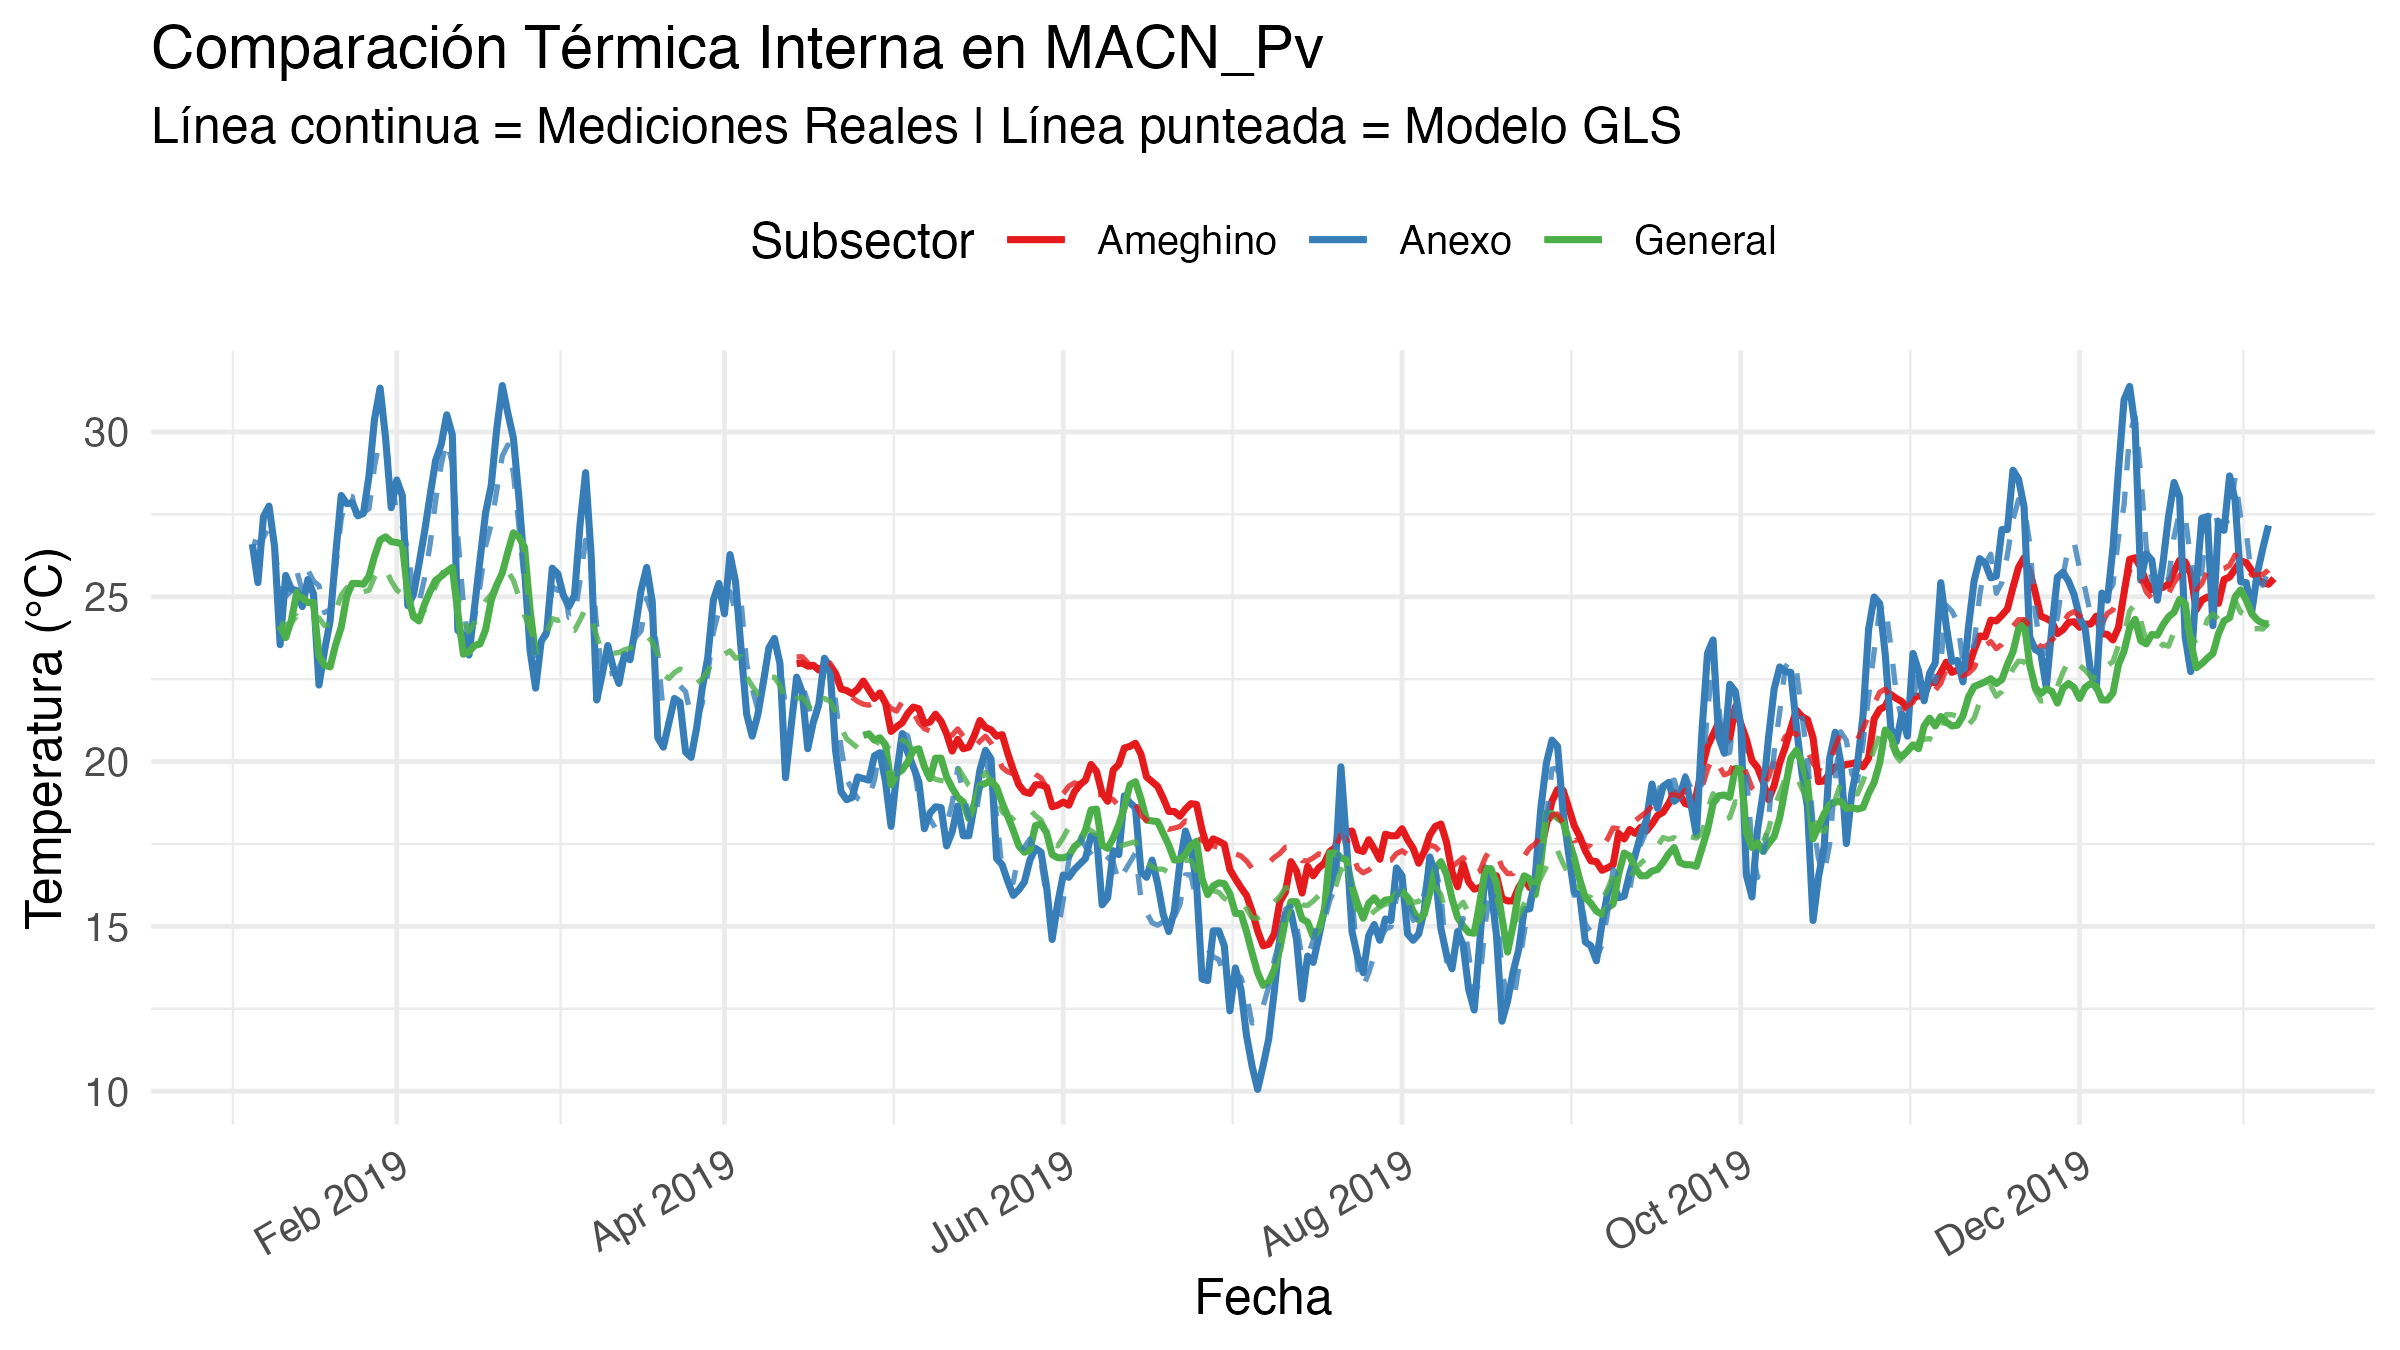
\includegraphics[width=0.88\textwidth]{fig_modelo_pv.png}
  \caption{Ajuste del modelo GLS en Paleovertebrados (MACN\_Pv). Línea continua: mediciones observadas; línea punteada: predicción del modelo GLS.}
  \label{fig:modelo_pv}
\end{figure}

\subsection{Dinámica de insectos plaga y condiciones ambientales}
El análisis exploratorio de las trampas de coleópteros y lepidópteros indica una clara correspondencia entre las temperaturas estivales y el incremento en las tasas de captura (Figura~\ref{fig:trampas_temp}).

\begin{figure}[htbp]
  \centering
  % Ancho ajustado proporcionalmente sin deformación
  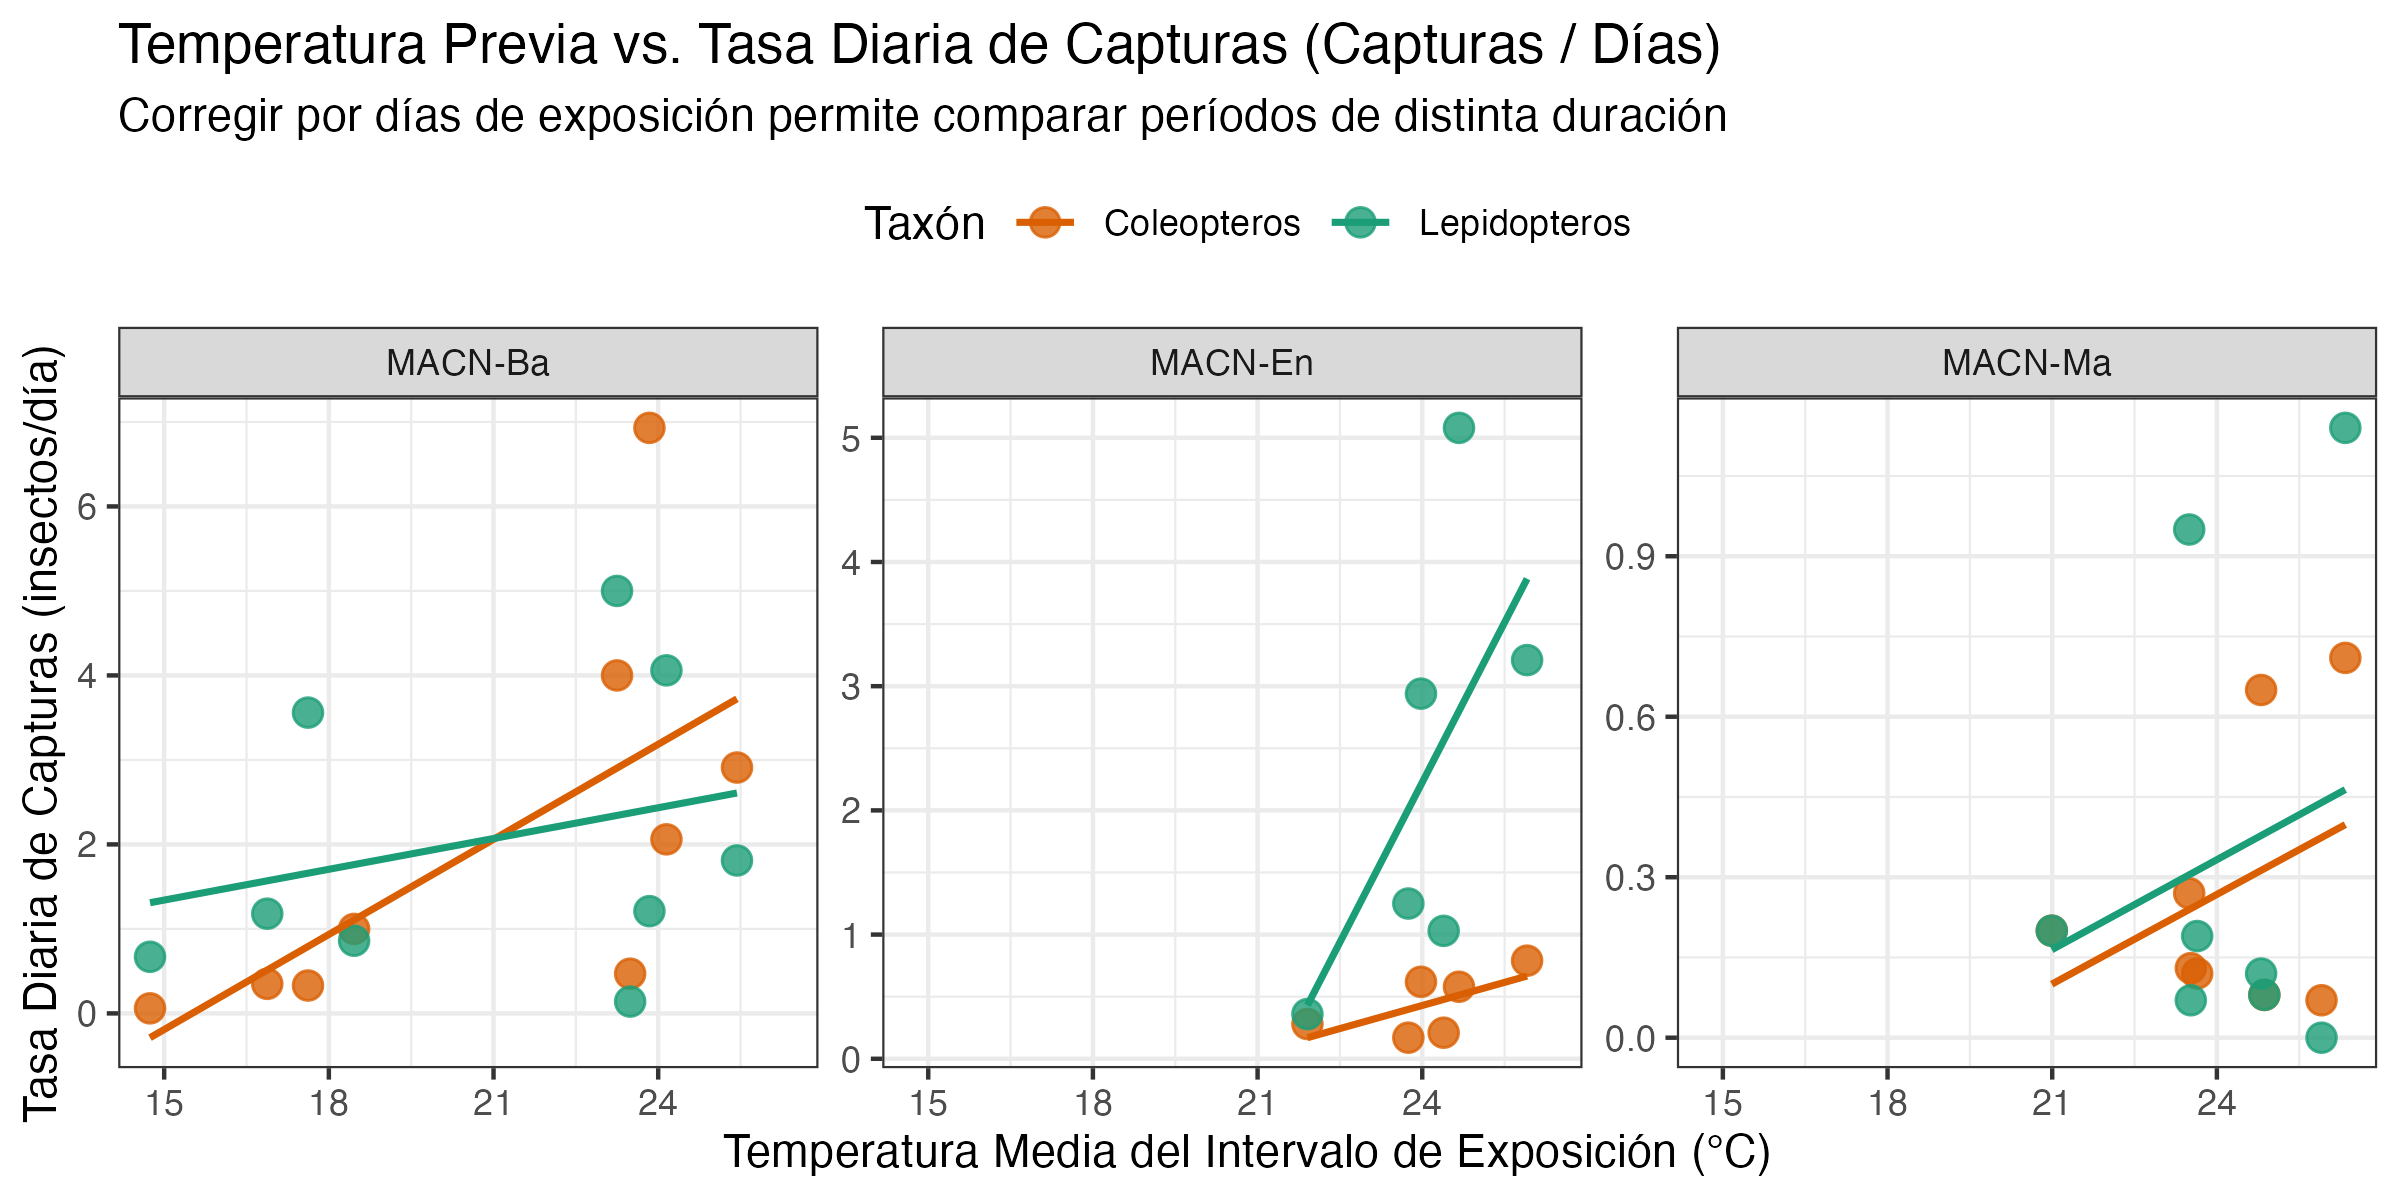
\includegraphics[width=0.88\textwidth]{fig_trampas_temperatura.png}
  \caption{Relación entre la temperatura previa y la tasa diaria de capturas por sala y taxón. La normalización por días de exposición permite comparar períodos de diferente duración.}
  \label{fig:trampas_temp}
\end{figure}

% ==============================================================================
% 6. DISCUSIÓN Y CONCLUSIONES
% ==============================================================================
\section{Discusión y Conclusiones}

\subsection{Interpretación disciplinar y recomendaciones}
Se identifican dos tipologías edilicias en el museo: salas expuestas que requieren refuerzo de aislamiento térmico, y salas protegidas que mantienen una elevada estabilidad pasiva...

\subsection{Limitaciones del estudio}
Es necesario señalar que el muestreo de trampas biológicas presentó revisiones muy espaciadas e intervalos desiguales (desde 9 hasta 161 días), lo cual restringe la posibilidad de predecir capturas en horizontes de corto plazo. No obstante, el control por tiempo de exposición mediante modelos con offset permite extraer conclusiones válidas sobre la estacionalidad del riesgo...

% ==============================================================================
% 7. REFERENCIAS BIBLIOGRÁFICAS
% ==============================================================================
\section{Referencias}
\begin{itemize}
    \item Pinheiro, J. C., \& Bates, D. M. (2000). \textit{Mixed-effects models in S and S-PLUS}. Springer.
    \item R Core Team (2023). \textit{R: A language and environment for statistical computing}. R Foundation for Statistical Computing, Vienna, Austria.
    \item Thomson, G. (1986). \textit{The Museum Environment}. Butterworth-Heinemann.
\end{itemize}

% ==============================================================================
% 8. ANEXOS (Opcional, máximo 5 carillas)
% ==============================================================================
\appendix
\section{Anexos}
Diagnósticos complementarios de residuos y tablas auxiliares...

\end{document}
